% =====================================================================
% Documentación técnica formal — Proyecto Capstone "Evento Cultural"
% Compilación: pdflatex -interaction=nonstopmode main.tex  (dos pasadas)
% =====================================================================
\documentclass[11pt,a4paper]{article}

\usepackage[utf8]{inputenc}
\usepackage[T1]{fontenc}
\usepackage[spanish]{babel}
\usepackage{lmodern}
\usepackage[margin=2.4cm]{geometry}
\usepackage{graphicx}
\usepackage{xcolor}
\usepackage{booktabs}
\usepackage{longtable}
\usepackage{array}
\usepackage{enumitem}
\usepackage{caption}

\definecolor{terracota}{HTML}{C9622D}
\definecolor{verdes}{HTML}{1F5C57}
\definecolor{rojo}{HTML}{B03A3A}
\definecolor{azulurl}{HTML}{1F4E79}
\usepackage[colorlinks=true,linkcolor=azulurl,urlcolor=azulurl]{hyperref}

\graphicspath{{Diagramas/}}
\captionsetup{font=small,labelfont=bf}
\renewcommand{\tablename}{Tabla}

\newcommand{\pendiente}{\textcolor{rojo}{\textbf{Pendiente de completar por el equipo.}}}
\newcommand{\seccionpendiente}[1]{\textcolor{rojo}{\textbf{Pendiente de completar por el equipo:} #1}}

\title{}
\author{}
\date{}

\begin{document}

% ---------------------------------------------------------- PORTADA
\begin{titlepage}
\centering
{\color{terracota}\rule{\textwidth}{2pt}}\\[0.6cm]
{\Large \textsc{Duoc UC -- Sede Maipú}}\\[0.2cm]
{\large Capstone 2026 -- Asignatura APT122}\\[1.4cm]
{\color{terracota}\Huge \textbf{Evento Cultural}}\\[0.5cm]
{\LARGE Documentación Técnica del Proyecto}\\[0.4cm]
{\large Plataforma chilena de eventos culturales}\\[1.2cm]
{\color{terracota}\rule{\textwidth}{1pt}}\\[1.2cm]

\begin{minipage}{0.82\textwidth}
\renewcommand{\arraystretch}{1.35}
\begin{center}
\begin{tabular}{>{\bfseries}l l}
Integrante & Rol principal \\ \midrule
Roberto Riffo & Líder de proyecto / Frontend / UX \\
José Miguel Moncada & Base de datos / QA \\
David Herrera & Backend e integraciones \\
\end{tabular}
\end{center}
\vspace{0.2cm}
{\small Roles según el design brief aprobado en Fase 1 (\textit{design\_brief\_capstone.docx}).}
\end{minipage}

\vspace{1.2cm}
\begin{minipage}{0.82\textwidth}
\small
\textbf{Stack del sistema:} Python (scraper con conectores, NVIDIA NIM y checkpoints SQLite),
Supabase/PostgreSQL con Row Level Security, Angular 22 + Ionic 9 (web y móvil),
GitHub Actions para automatización.
\end{minipage}

\vfill
{\large Versión 1.0}\\[0.2cm]
{\large 24 de septiembre de 2026}\\[0.4cm]
{\small Documento elaborado exclusivamente con evidencia verificable del repositorio.\\
Las omisiones se declaran como \textcolor{rojo}{\textbf{pendientes del equipo}} y están
trazadas en el \textit{Registro de Cambios de Documentación}.}\\[0.3cm]
{\color{terracota}\rule{\textwidth}{2pt}}
\end{titlepage}

% ---------------------------------------------------------- ÍNDICE
\tableofcontents
\newpage

% ---------------------------------------------------------- INTRODUCCIÓN
\section{Introducción y alcance}
\label{sec:intro}

Este documento consolida la documentación técnica formal del proyecto \textbf{Evento
Cultural}, una plataforma chilena para compilar y difundir eventos culturales, comerciales
y municipales. Fue elaborado a partir de la evidencia disponible en el propio repositorio:
el código y la documentación interna del scraper (\texttt{Scraper de eventos culturales.rar}),
el código y la documentación del frontend (\texttt{evento-cultural.rar}), el modelo de base
de datos (DBML, migraciones documentadas y diccionario de tablas), los requerimientos
priorizados en Fase 1 (matriz MoSCoW) y el diagrama de arquitectura de Fase 2.

\textbf{Convención de honestidad documental:} este documento distingue explícitamente entre
lo \emph{implementado} (respaldado por código), lo \emph{parcial} (respaldado solo en parte)
y lo \emph{pendiente} (información humana o trabajo futuro). Nada se afirma como terminado
sin respaldo; los puntos abiertos se marcan con \pendiente

\subsection{Estructura del sistema}

El sistema se compone de tres bloques independientes que se comunican a través de la base
de datos: el \textbf{scraper} (recolección y enriquecimiento de datos), la \textbf{base de
datos} (catálogo canónico en Supabase/PostgreSQL) y el \textbf{frontend} (aplicación web y
móvil), con \textbf{GitHub Actions} como automatización de la ejecución del scraper
(ver Figura~\ref{fig:arq} en la Sección~\ref{sec:arq}).

% =====================================================================
% PARTE 1 — Arquitecturas (general, scraper, frontend)
% =====================================================================

\section{Arquitectura general del sistema}
\label{sec:arq}

\subsection{Visión general}

El sistema sigue una arquitectura de tres bloques desacoplados que se comunican a través de
la base de datos, más un actor de automatización:

\begin{itemize}[leftmargin=1.4em]
    \item \textbf{Scraper (Python):} recolecta eventos desde fuentes públicas chilenas,
    los normaliza y los enriquece selectivamente con NVIDIA NIM.
    \item \textbf{Base de datos (Supabase/PostgreSQL):} catálogo canónico con Row Level
    Security, bitácora de ejecuciones y evidencia de extracción.
    \item \textbf{Frontend (Angular 22 + Ionic 9):} aplicación web y móvil para descubrir,
    filtrar y publicar eventos.
    \item \textbf{GitHub Actions:} automatiza la ejecución del scraper, ejecuta las pruebas
    y sincroniza la base de datos.
\end{itemize}

\begin{figure}[ht]
\centering
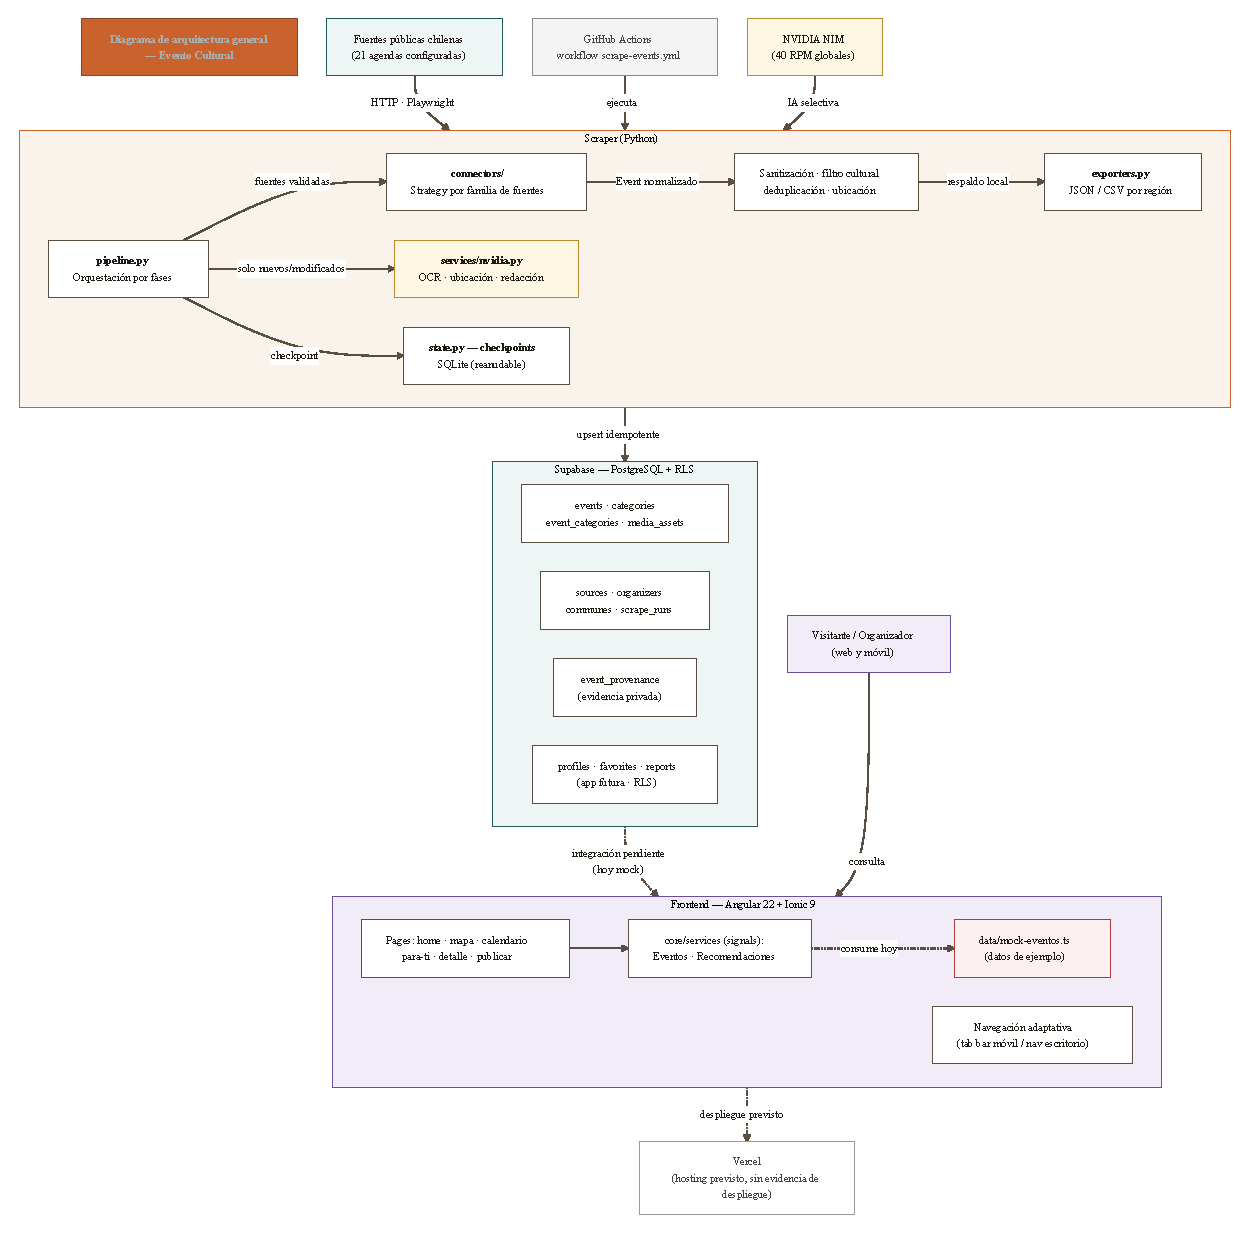
\includegraphics[width=\textwidth]{01_arquitectura_general.pdf}
\caption{Arquitectura general del sistema (fuente editable: \texttt{Diagramas/01\_arquitectura\_general.mmd}, Mermaid).}
\label{fig:arq}
\end{figure}

\subsection{Comunicación entre servicios}

\begin{table}[ht]
\centering\small
\renewcommand{\arraystretch}{1.25}
\begin{tabular}{p{3.4cm} p{4.0cm} p{7.4cm}}
\toprule
\textbf{Origen $\rightarrow$ Destino} & \textbf{Mecanismo} & \textbf{Detalle} \\
\midrule
GitHub Actions $\rightarrow$ Scraper & Ejecución de \texttt{scrape\_events.py} & Fases separables (\texttt{-{}-phase extract} / \texttt{-{}-phase process}); estado restaurado por artefactos \\
Scraper $\rightarrow$ Fuentes & HTTP directo o Playwright & Caché condicional (ETag/Last-Modified), límites por dominio, respeto de \texttt{robots.txt} y \texttt{Retry-After} \\
Scraper $\rightarrow$ NVIDIA NIM & API de inferencia & Limitador global de 40 RPM con reintentos \\
Scraper $\rightarrow$ SQLite & Checkpoints por fuente y ficha & Reanudación de OCR/IA pendiente en futuras ejecuciones \\
Scraper $\rightarrow$ Supabase & API REST (upserts idempotentes) & Carga por lotes (\texttt{SUPABASE\_BATCH\_SIZE}); borrado de vencidos y conciliación configurables \\
Frontend $\rightarrow$ Supabase & Cliente/API REST & \textbf{Pendiente:} hoy consume datos de ejemplo en memoria \\
\bottomrule
\end{tabular}
\caption{Comunicación entre servicios del sistema.}
\label{tab:com}
\end{table}

Cada fuente se procesa de manera independiente: si una falla, las demás continúan. Solo se
publican eventos vigentes; la conciliación retira registros antiguos únicamente cuando la
extracción fue completa y segura (diagrama de arquitectura de Fase 2).

\subsection{Estado de la integración frontend--base de datos}

El frontend entregado funciona con \textbf{datos de ejemplo en memoria}
(\texttt{src/app/data/mock-eventos.ts}) según su propio README; los formularios de inicio de
sesión y publicación simulan el flujo. La documentación del scraper y del frontend define el
punto de integración futuro (\texttt{EventosService}). \seccionpendiente{cronograma y
responsables de la conexión real a Supabase y de la autenticación real.}

\section{Arquitectura del scraper}
\label{sec:scraper}

\subsection{Modelo general}

Pipeline por fases con conectores intercambiables. Los ejecutables de la raíz
(\texttt{scrape\_events.py}, \texttt{add\_source.py}, \texttt{validate\_sources.py}) reciben
la orden; el trabajo reside en el paquete \texttt{eventos/}. El flujo principal, según
\texttt{docs/ARCHITECTURE.md}, es:

\begin{enumerate}[leftmargin=1.6em]
    \item \texttt{SourceRepository} carga y valida los archivos de \texttt{sources/}.
    \item El pipeline agrupa fuentes por dominio y las procesa con un pool acotado.
    \item \texttt{ConnectorFactory} selecciona una Strategy según el campo \texttt{connector};
    cada conector devuelve objetos \texttt{Event} con el mismo esquema.
    \item \texttt{EventSanitizer} limpia los campos, limita descripciones y descarta vencidos.
    \item Deduplicación por fuente y global, fijando el identificador estable.
    \item \texttt{LocationNormalizer} aplica valores por defecto, reglas y, solo si falta
    información, IA.
    \item Filtro regional y ubicación canónica.
    \item \texttt{DatasetExporter} escribe el respaldo local (JSON/CSV por región).
    \item Si Supabase está habilitado, \texttt{SupabaseExporter} sincroniza con upserts
    idempotentes y elimina vencidos remotos.
\end{enumerate}

\subsection{Conectores y fuentes}

\begin{table}[ht]
\centering\small
\renewcommand{\arraystretch}{1.2}
\begin{tabular}{l p{9.2cm}}
\toprule
\textbf{Conector} & \textbf{Uso} \\
\midrule
\texttt{wordpress\_rest} & APIs WordPress REST con \texttt{field\_map} declarativo \\
\texttt{json\_api} & APIs JSON genéricas con paginación \\
\texttt{json\_ld} & Sitios con datos estructurados Schema.org \\
\texttt{html\_cards} & Carteleras HTML estáticas con selectores CSS declarativos \\
\texttt{eventon}, \texttt{tribe} & Plugins de eventos (EventON, The Events Calendar) \\
\texttt{ticketplus}, \texttt{maipu}, \texttt{fisa} & Conectores especializados \\
\texttt{generic} & Busca JSON-LD primero; usa NVIDIA NIM solo si faltan datos estructurados \\
\bottomrule
\end{tabular}
\caption{Conectores disponibles en el paquete \texttt{eventos/connectors/}.}
\label{tab:conn}
\end{table}

Las fuentes se declaran en \texttt{sources/*.json}: 20 permanentes más 1 estacional de
septiembre (tabla completa en el README del scraper), con plantillas por familia en
\texttt{sources/templates/}.

\subsection{Enriquecimiento selectivo con NVIDIA NIM}

Solo los eventos nuevos o modificados pasan por OCR, normalización de ubicación y redacción
editorial; los eventos sin cambios se reutilizan por hash de entrada. Las tareas pendientes
quedan en la cola persistente del checkpoint SQLite y se recuperan en ejecuciones futuras.
El limitador global \texttt{NVIDIA\_RPM\_LIMIT=40} espacia las peticiones aunque varios
conectores terminen simultáneamente.

\subsection{Pipeline reanudable y concurrencia}

Cada fuente y resultado de IA se guarda en \texttt{state/pipeline.sqlite3} (ver
\texttt{docs/RESUMABLE\_PIPELINE.md}). El workflow de GitHub Actions restaura y conserva este
estado mediante artefactos. Con \texttt{SOURCE\_WORKERS=4} se crean trabajadores internos;
las fuentes de un mismo dominio se procesan en serie (\emph{bulkhead} por dominio) y la
salida es determinista. La caché HTTP condicional persistente (ETag/Last-Modified) evita
descargas innecesarias.

\subsection{Patrones de diseño aplicados}

Strategy (conectores), Registry/Factory, Repository, inyección de dependencias para pruebas,
Adapter (\texttt{SupabaseExporter}), Chain of Responsibility (ubicación), Rate Limiter global
(NVIDIA), Bulkhead por dominio, Cache-Aside condicional y post-processing pipeline
obligatorio de saneamiento y vigencia (un conector nuevo no puede saltárselo).

\subsection{Pendientes de la arquitectura del scraper}

\begin{itemize}[leftmargin=1.4em]
    \item La periodicidad del workflow quedó resuelta: el bloque \texttt{schedule}
    está activo desde el 24-09-2026 con cron diario a las 00:37 (America/Santiago),
    verificado en GitHub Actions (corridas \#9--\#11 del 25 al 27-09-2026). Queda como
    mejora pendiente congelar el reloj en las pruebas de vigencia para que las corridas
    programadas no fallen por fechas simuladas vencidas (ver sección de pruebas).
    \seccionpendiente{primera ejecución automática completa con la suite en verde.}
    \item La carpeta \texttt{supabase/} con las migraciones SQL no está incluida en la copia
    entregada (la documentación la referencia). \seccionpendiente{confirmar su presencia en
    el repositorio oficial.}
\end{itemize}

\section{Arquitectura del frontend}
\label{sec:frontend}

\subsection{Stack real}

\begin{table}[ht]
\centering\small
\renewcommand{\arraystretch}{1.2}
\begin{tabular}{l l}
\toprule
\textbf{Componente} & \textbf{Versión} \\
\midrule
Angular & 22.0.1 (componentes standalone, sin NgModules) \\
Ionic Framework & \textasciicircum 9.0.0 \\
Capacitor & 8.x (app, haptics, keyboard, status-bar) \\
TypeScript & \textasciitilde 6.0.0 \\
Pruebas & Vitest \textasciicircum 4.0.8 (con jsdom) \\
Lint & ESLint \textasciicircum 9.16.0 + angular-eslint 22.0.0 \\
\bottomrule
\end{tabular}
\caption{Stack del frontend según \texttt{package.json}.}
\label{tab:stack}
\end{table}

\subsection{Estructura y navegación}

La aplicación organiza el código en \texttt{core/} (modelos \texttt{Evento} y
\texttt{Recomendacion}; servicios con signals: \texttt{EventosService},
\texttt{RecomendacionService}, \texttt{ToastService} y \texttt{ViewPreferencesService}),
\texttt{features/home/} (descubrimiento y layouts de inicio), \texttt{layout/}
(\texttt{MainLayoutComponent}) y \texttt{pages/}. Las rutas registradas
(\texttt{app.routes.ts}) son: \texttt{/home}, \texttt{/para-ti}, \texttt{/calendario},
\texttt{/mapa}, \texttt{/evento/:id}, \texttt{/publicar}, \texttt{/perfil} y \texttt{/login},
con redirecciones de compatibilidad (\texttt{/buscar} y \texttt{/favoritos}).

La navegación es adaptativa sin JavaScript adicional: tab bar inferior en móvil y barra
superior en escritorio, ambas dentro de \texttt{MainLayoutComponent} mediante las clases
responsive de Ionic. La identidad visual (paleta terracota/verde/ámbar y tipografías
Fraunces/Inter) está centralizada en \texttt{src/theme/variables.scss}.

\begin{figure}[ht]
\centering
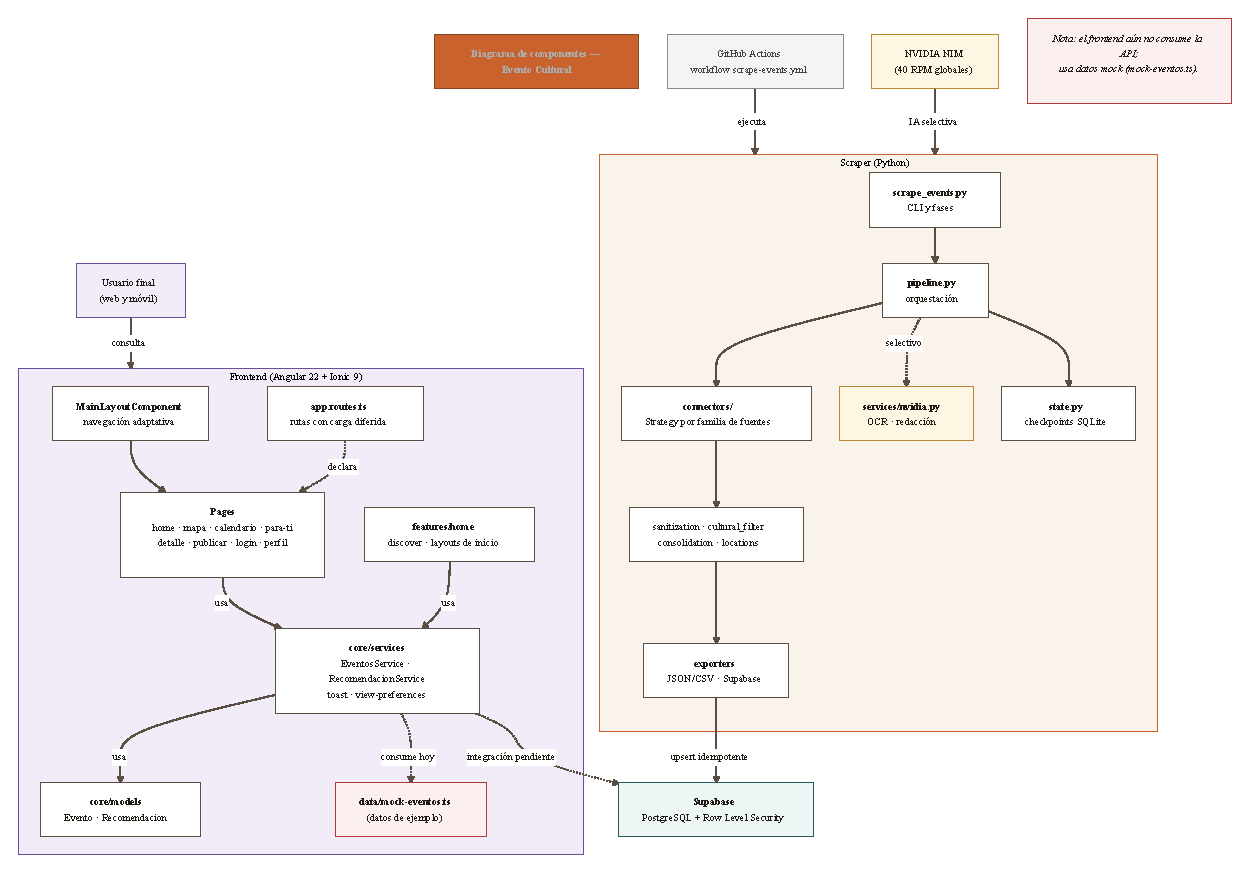
\includegraphics[width=0.92\textwidth]{02_componentes.pdf}
\caption{Diagrama de componentes del sistema (fuente editable: \texttt{Diagramas/02\_componentes.mmd}, Mermaid).}
\label{fig:comp}
\end{figure}

\subsection{Filtros y funcionalidad}

\texttt{EventosService} implementa orden por fecha, nombre, categoría, cercanía y
actualización, y filtros combinables: texto, categorías múltiples, región, comuna, rango de
fechas, gratuito, modalidad (presencial/virtual/híbrido), público objetivo y accesibilidad.
La vista ``para ti'' (\texttt{RecomendacionService}) sustituyó a favoritos como experiencia
de recomendación.

\subsection{Estrategia de despliegue}

Decisión del equipo (comunicada el 24-09-2026), consistente con el stack definido en Fase 1:

\begin{itemize}[leftmargin=1.4em]
    \item \textbf{Web:} despliegue en \textbf{Vercel} (ya figuraba como hosting previsto en
    el design brief de Fase 1). A la fecha no existe evidencia de un despliegue ejecutado.
    \item \textbf{Android:} la aplicación móvil se compila con \textbf{Capacitor 8}
    (dependencias presentes en \texttt{package.json}) y \textbf{Android Studio}.
    \item \textbf{Scraper:} automatización con \textbf{GitHub Actions} (workflow
    \texttt{scrape-events.yml}).
    \item \textbf{No se utilizará Docker} como mecanismo de despliegue
    (ver Sección~\ref{sec:docker}).
\end{itemize}

\subsection{Pendientes del frontend}

\seccionpendiente{conexión real a Supabase (sustituir los datos mock por el cliente de la
API), activación de la autenticación real y persistencia de favoritos del usuario.}

% =====================================================================
% PARTE 2 — Modelo de datos y diagramas UML
% =====================================================================

\section{Modelo de datos (Supabase / PostgreSQL)}
\label{sec:datos}

\subsection{Fuente del modelo}

El modelo se documenta a partir de \texttt{docs/DATABASE.md}, \texttt{docs/SUPABASE.md},
el DBML editable (\texttt{docs/evento\_cultural\_modelo.dbml}), el diccionario de tablas
(DOCX, versión documentada al 21-09-2026) y el diagrama ER de Fase 1
(\texttt{DB\_evento\_cultural.pdf}). \seccionpendiente{la carpeta \texttt{supabase/migrations/}
con los archivos SQL no está incluida en la copia entregada; confirmar su presencia en el
repositorio oficial.}

\begin{figure}[ht]
\centering
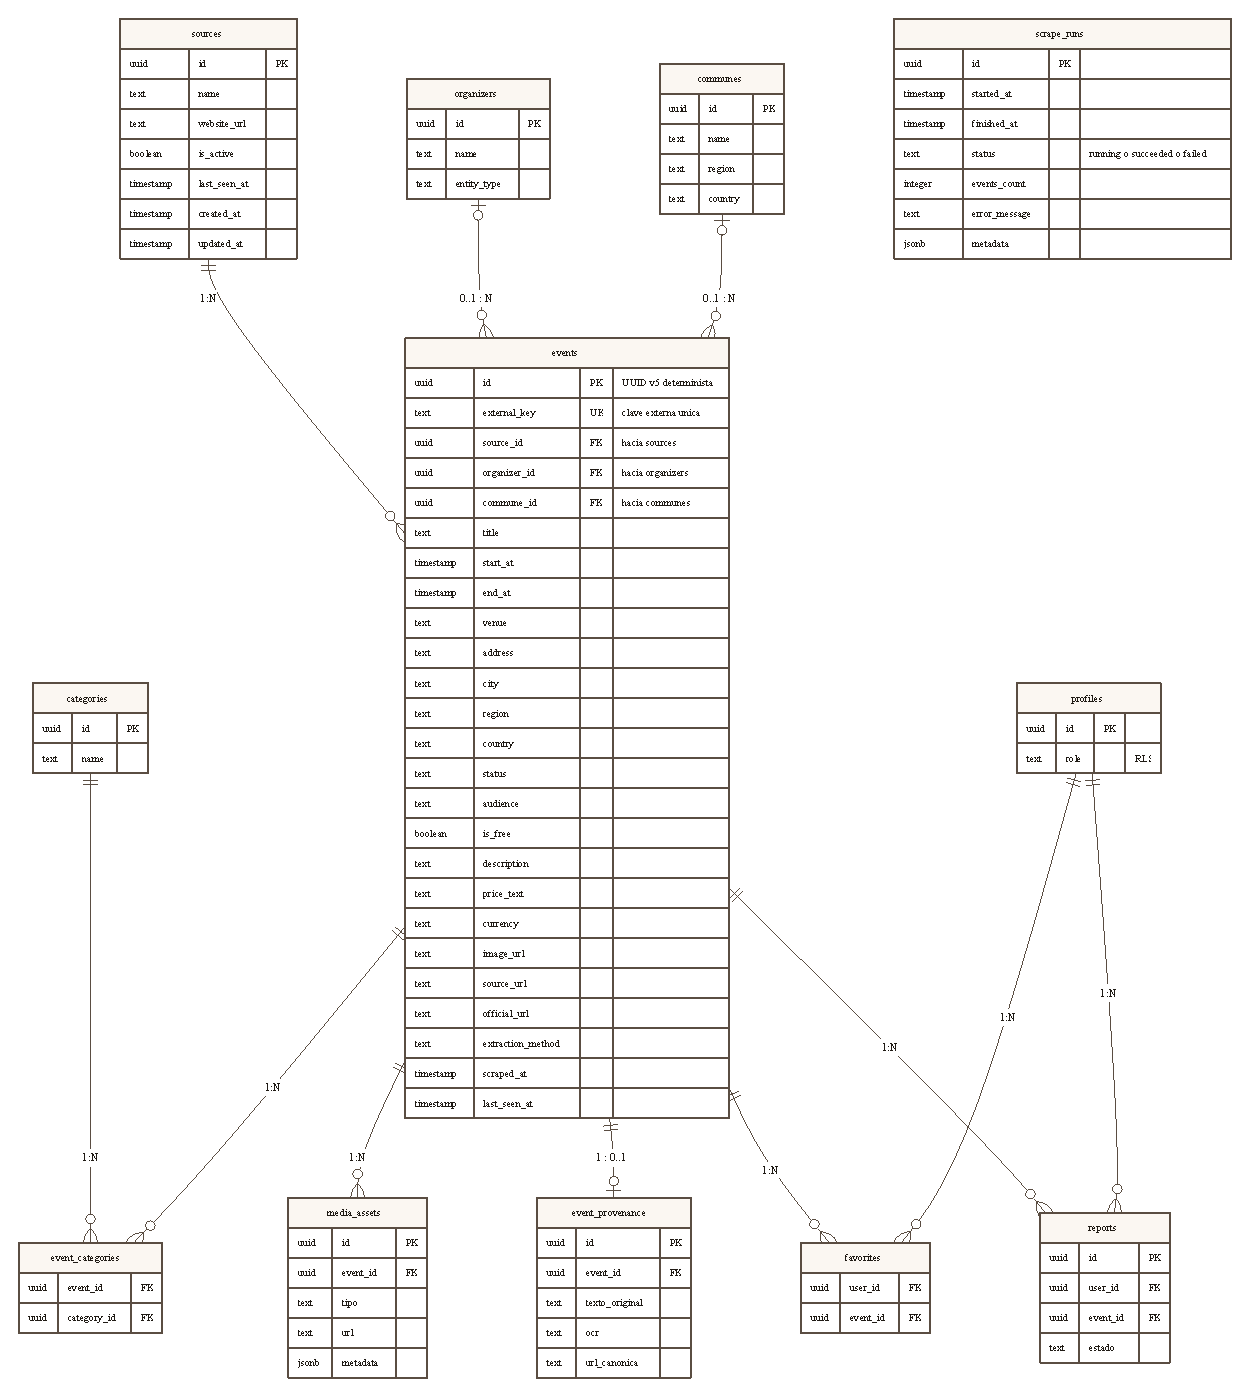
\includegraphics[width=0.95\textwidth]{06_modelo_er.pdf}
\caption{Modelo entidad--relación (fuente editable: \texttt{Diagramas/06\_modelo\_er.mmd}, Mermaid).}
\label{fig:er}
\end{figure}

\subsection{Tablas y finalidad}

\begin{table}[ht]
\centering\small
\renewcommand{\arraystretch}{1.25}
\begin{tabular}{l p{4.1cm} p{6.6cm}}
\toprule
\textbf{Grupo} & \textbf{Tabla} & \textbf{Finalidad} \\
\midrule
Ingesta y catálogo & \texttt{sources} & Agenda, municipalidad, ticketera o sitio de origen \\
 & \texttt{organizers} & Institución responsable del evento \\
 & \texttt{communes} & Ubicación administrativa normalizada \\
 & \texttt{categories} & Etiquetas temáticas, de formato o audiencia \\
 & \texttt{events} & Registro canónico del evento consolidado (37 columnas) \\
 & \texttt{event\_categories} & Relación N:M entre eventos y categorías \\
 & \texttt{media\_assets} & Imágenes y futuros multimedia \\
 & \texttt{scrape\_runs} & Bitácora de ejecuciones locales y de GitHub Actions \\
 & \texttt{event\_provenance} & Evidencia privada: texto original, OCR y URL canónica \\
Aplicación futura & \texttt{profiles}, \texttt{favorites}, \texttt{reports} & Base prevista de la aplicación; no intervienen en el scraper \\
\bottomrule
\end{tabular}
\caption{Tablas del modelo de datos según el diccionario y el DBML del proyecto.}
\label{tab:tablas}
\end{table}

Los identificadores de eventos, organizadores, comunas y categorías son \textbf{UUID v5
deterministas} derivados de claves externas: ejecutar dos veces el mismo scraping actualiza
las filas (upsert) sin crear duplicados. El campo \texttt{categories} se normaliza en
\texttt{categories} y \texttt{event\_categories}, conservando la relación muchos-a-muchos.

\subsection{Seguridad (Row Level Security) y ciclo de carga}

La migración de RLS habilita Row Level Security en todas las tablas; \texttt{scrape\_runs}
no tiene lectura pública; el usuario no puede cambiar su propio rol ni el estado de sus
reportes desde el frontend; la vista \texttt{public\_event\_catalog} hereda las reglas RLS y
no expone eventos suprimidos ni organizadores bloqueados.

En el ciclo de carga, la sincronización identifica coincidencias por URL o clave compuesta,
carga por lotes (\texttt{SUPABASE\_BATCH\_SIZE}) y registra cada ejecución en
\texttt{scrape\_runs} como \texttt{running}, \texttt{succeeded} o \texttt{failed}. La
repetición idempotente es el mecanismo de recuperación ante cargas parciales.

\subsection{Limitaciones declaradas}

Sin marca explícita de eventos de día completo; \texttt{price\_text} no permite comparación
numérica; categorías sin jerarquía almacenada; registros de Chile Cultura que pueden ser
directorios y no eventos fechados; etiqueta inválida conocida (\texttt{Calendar\_Month
Inscribirse}); borrado físico de vencidos solo con
\texttt{SUPABASE\_DELETE\_EXPIRED=true}.

\section{Diagramas UML}
\label{sec:uml}

Los cuatro diagramas UML exigidos por el anexo metodológico se escriben como código fuente
Mermaid (\texttt{.mmd}) y se renderizan a PDF con \texttt{mermaid-cli}, en la carpeta
\texttt{Diagramas/} de esta misma sección. Los casos de uso se derivan de la matriz MoSCoW de
Fase 1 y de las páginas realmente implementadas en el frontend. Todos los diagramas (01--06)
comparten un estándar visual único (paleta institucional, tipografía Arial, flechas
reforzadas), declarado dentro de cada archivo \texttt{.mmd}, y fueron regenerados el
27-09-2026 al migrar de Draw.io a Mermaid para automatizar el trazado de líneas y facilitar
el mantenimiento (detalle en el \texttt{REGISTRO\_CAMBIOS\_DOCUMENTACION.md}, §16.3).

\subsection{Casos de uso}

\begin{figure}[ht]
\centering
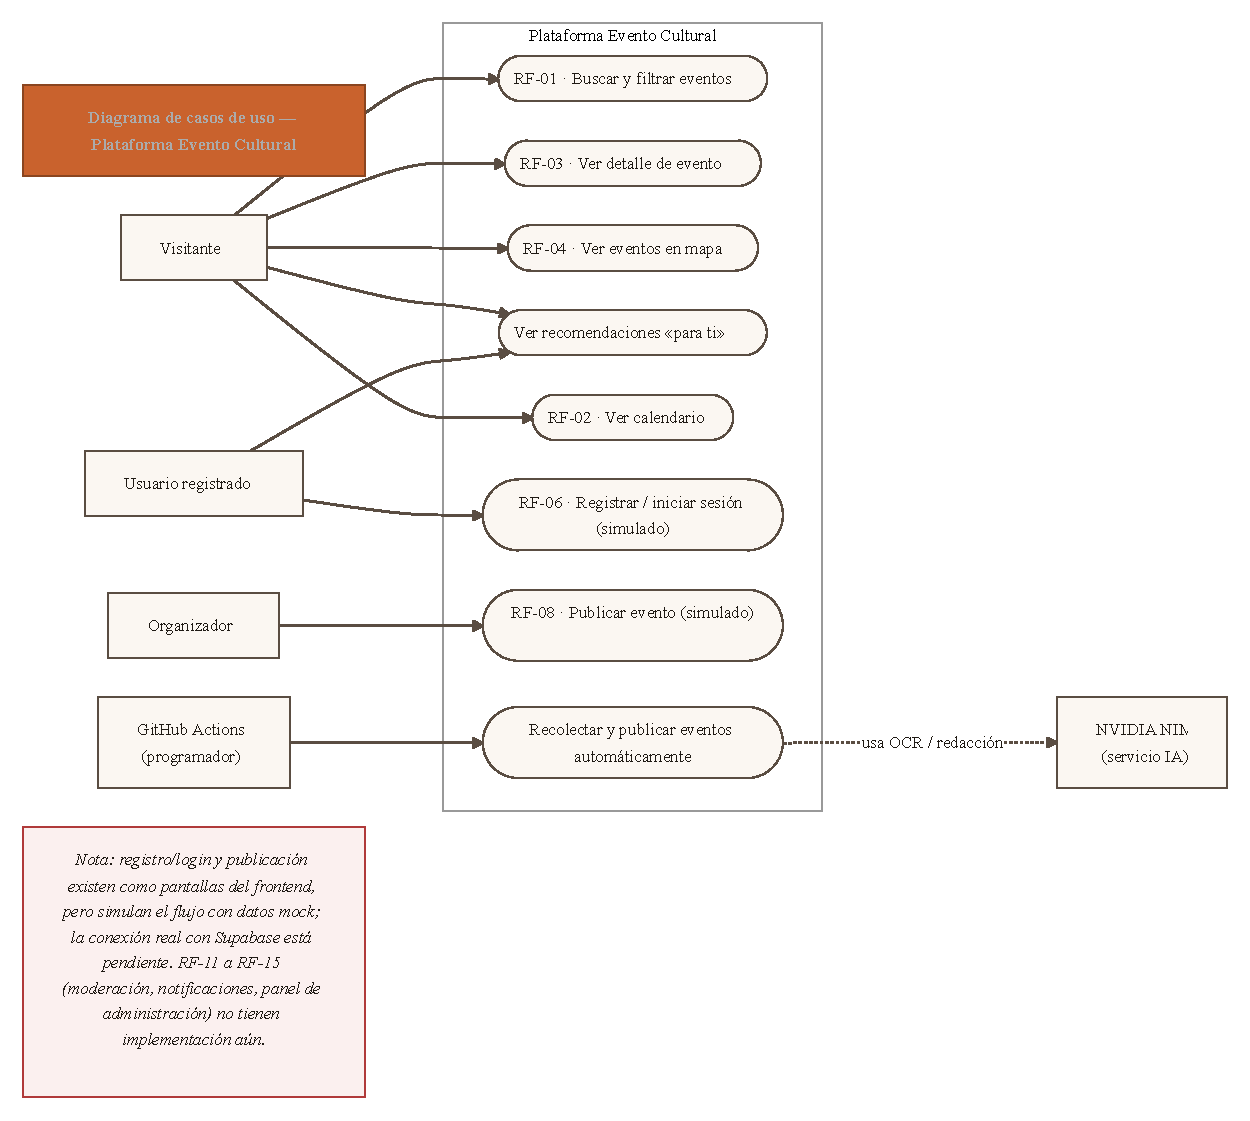
\includegraphics[width=0.9\textwidth]{03_casos_de_uso.pdf}
\caption{Casos de uso de la plataforma (fuente editable: \texttt{Diagramas/03\_casos\_de\_uso.mmd}, Mermaid).}
\label{fig:uc}
\end{figure}

El visitante busca, filtra, ve el detalle, consulta el mapa y el calendario; el usuario
registrado inicia sesión y recibe recomendaciones; el organizador publica eventos
(simulado); GitHub Actions activa la recolección automática, que usa NVIDIA NIM como
servicio externo de OCR y redacción.

\subsection{Secuencia de la funcionalidad principal}

\begin{figure}[ht]
\centering
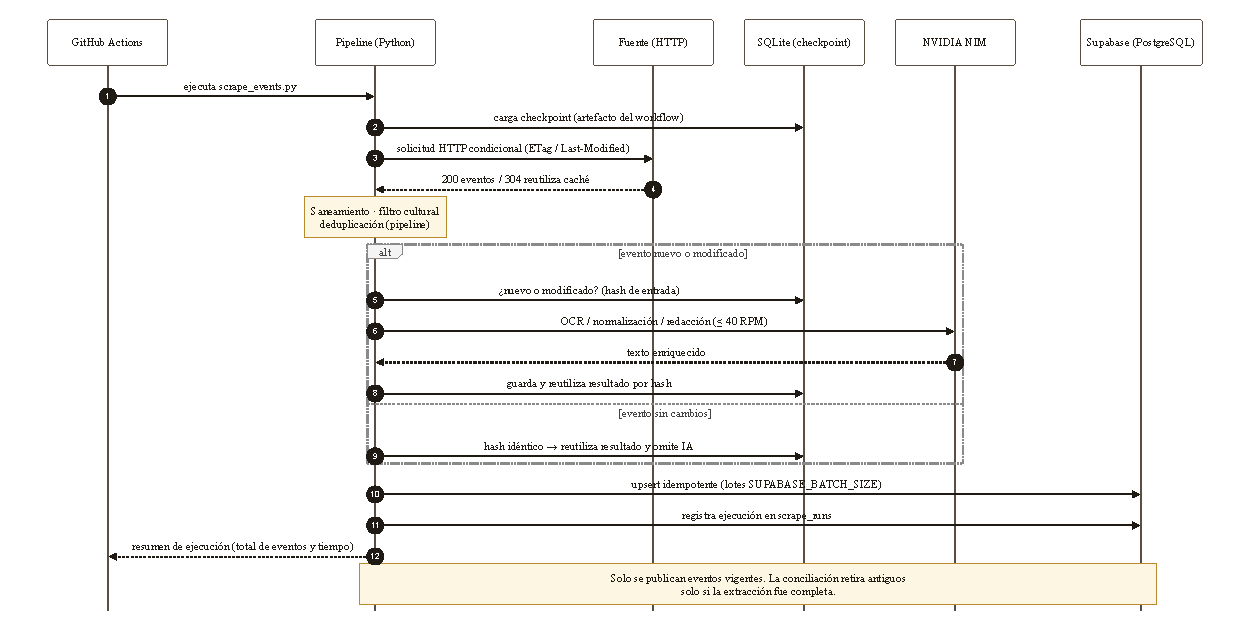
\includegraphics[width=\textwidth]{04_secuencia.pdf}
\caption{Secuencia: extracción, enriquecimiento y publicación (editable: \texttt{Diagramas/04\_secuencia.mmd}, Mermaid).}
\label{fig:seq}
\end{figure}

El flujo principal del sistema es la obtención y publicación de eventos: GitHub Actions
ejecuta el pipeline; este restaura el checkpoint, consulta las fuentes con caché
condicional, sanea y deduplica, decide mediante hash qué eventos pasan por IA (con límite
de 40 RPM), reutiliza resultados previos y sincroniza Supabase con upserts idempotentes,
registrando la corrida en \texttt{scrape\_runs}.

\subsection{Componentes y clases}

El diagrama de componentes (Figura~\ref{fig:comp}) muestra los módulos del frontend y del
scraper y su comunicación con la base de datos. El diagrama de clases (conceptual) refleja
los roles reales del núcleo del scraper documentados en \texttt{docs/ARCHITECTURE.md}:
\texttt{EventPipeline}, \texttt{ConnectorFactory}, \texttt{Connector} (Strategy),
\texttt{Event}, \texttt{EventSanitizer}, \texttt{LocationNormalizer},
\texttt{NvidiaService}, \texttt{SupabaseExporter}, \texttt{DatasetExporter} y
\texttt{PipelineState}.

\begin{figure}[ht]
\centering
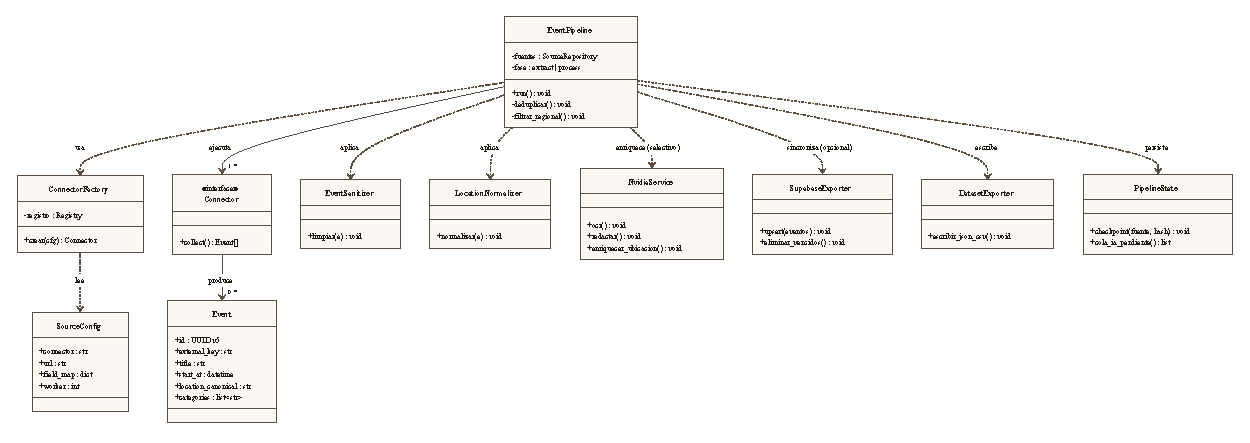
\includegraphics[width=0.95\textwidth]{05_clases.pdf}
\caption{Diagrama de clases conceptual del núcleo del scraper (editable: \texttt{Diagramas/05\_clases.mmd}, Mermaid).}
\label{fig:cls}
\end{figure}

\subsection{Pendientes de UML}

\seccionpendiente{si el docente exige una versión gráfica adicional con notación UML estricta,
regenerarla a partir de los archivos editables entregados y sustituir las figuras
correspondientes.}

% =====================================================================
% PARTE 3 — RNF, pruebas, Docker e innovación
% =====================================================================

\section{Requisitos no funcionales}
\label{sec:rnf}

\subsection{Requisitos definidos en Fase 1 (MoSCoW)}

\begin{table}[ht]
\centering\small
\renewcommand{\arraystretch}{1.2}
\begin{tabular}{l l p{6.8cm} l}
\toprule
\textbf{ID} & \textbf{Categoría} & \textbf{Requerimiento} & \textbf{Prioridad} \\
\midrule
RNF-01 & Usabilidad & Interfaz clara para ciudadanos y organizadores & Must \\
RNF-02 & Compatibilidad & Diseño responsive / multiplataforma & Must \\
RNF-03 & Rendimiento & Tiempos de carga aceptables con alto volumen & Should \\
RNF-04 & Seguridad & Protección de datos en tránsito y reposo & Must \\
RNF-05 & Seguridad & Control de acceso por rol & Must \\
RNF-06 & Disponibilidad & Disponibilidad estable según hosting definido & Should \\
RNF-07 & Escalabilidad & Crecimiento sostenido de datos & Should \\
RNF-08 & Calidad de datos & Normalización y consistencia entre fuentes & Must \\
RNF-09 & Mantenibilidad & Código mantenible y documentado & Should \\
RNF-10 & Localización & Contenido en español y contexto chileno & Must \\
RNF-11 & Portabilidad & Despliegue reproducible (GitHub Actions) & Could \\
RNF-12 & Accesibilidad & Buenas prácticas de accesibilidad web & Could \\
\bottomrule
\end{tabular}
\caption{Requisitos no funcionales priorizados (matriz MoSCoW de Fase 1).}
\label{tab:rnf}
\end{table}

\subsection{Estado real por requisito}

\begin{longtable}{l l p{9.3cm}}
\toprule
\textbf{ID} & \textbf{Estado} & \textbf{Evidencia verificable} \\
\midrule
\endhead
RNF-01 & Parcial & Navegación adaptativa implementada; sin evaluación de usabilidad registrada. \textcolor{rojo}{\textbf{Pendiente.}} \\
RNF-02 & Cumplido & Ionic/Angular responsive; navegación dual móvil/escritorio (\texttt{MainLayoutComponent}), grid con breakpoints. \\
RNF-03 & Parcial & Caché condicional, bulkhead por dominio y checkpoints optimizan la extracción; falta medición de tiempos del frontend con datos reales. \textcolor{rojo}{\textbf{Pendiente.}} \\
RNF-04 & Parcial & RLS en todas las tablas y secretos solo en entorno/GitHub Secrets; las pantallas de login y registro aún son simuladas. \\
RNF-05 & Parcial & El modelo prevé roles (\texttt{profiles.role}) y reglas RLS; el control de acceso funcional en la aplicación está pendiente. \\
RNF-06 & Parcial & GitHub Actions con ejecución manual y cron diario activo desde el 24-09-2026 (verificado: corridas \#9--\#11 del 25 al 27-09). \textcolor{rojo}{\textbf{Pendiente:} ejecución automática completa en verde tras corregir la prueba dependiente del tiempo (Plan de pruebas §5.1).} \\
RNF-07 & Cumplido (diseño) & Paginación por página en conectores, upsert idempotente y SQLite como buffer. \\
RNF-08 & Cumplido (pipeline) & Sanitización, filtro cultural, normalización de ubicación, deduplicación y UUID deterministas. \\
RNF-09 & Cumplido & Documentación interna (\texttt{docs/}), patrones documentados y 14 módulos de pruebas. \\
RNF-10 & Cumplido & Contenido en español; división administrativa chilena (regiones/comunas). \\
RNF-11 & Parcial & Portabilidad adoptada por el equipo: GitHub Actions (scraper), Vercel (web) y Capacitor 8 + Android Studio (Android); sin Docker por decisión del equipo (ver Sección~\ref{sec:docker}). \\
RNF-12 & Parcial & Accesibilidad como criterio de filtro en el frontend; auditoría formal pendiente. \textcolor{rojo}{\textbf{Pendiente.}} \\
\bottomrule
\caption{Estado real de cada requisito no funcional.}
\label{tab:rnfestado}
\end{longtable}

\subsection{Requisitos declarados y no implementados}

Para evitar inconsistencias en la evaluación se declara explícitamente: no existe
autenticación real en el frontend (pantallas simuladas); las notificaciones (RF-13), el
panel de administración (RF-14) y la moderación (RF-11/RF-12 del catálogo funcional) no
tienen implementación en el código entregado; las estadísticas (RF-17) quedaron
\emph{Won't have} en Fase 1; Docker no está implementado y el equipo decidió no utilizarlo
(Sección~\ref{sec:docker}).

\subsection{Limitaciones técnicas del desarrollo}

El desarrollo se realiza en un contexto académico sin presupuesto, lo que impone dos
limitaciones operativas visibles en el diseño del sistema:

\begin{itemize}[leftmargin=1.4em]
    \item \textbf{Cuota de la capa gratuita de IA (principalmente tiempo):} el
    enriquecimiento con IA se apoya en \textbf{NVIDIA Build}, plataforma de prototipado
    con modelos en la nube de uso gratuito pero sujeto a una cuota global de
    \textbf{40 peticiones por minuto (RPM)}. Esta restricción de tiempo condiciona el
    volumen de eventos que pueden procesarse por corrida y explica dos decisiones de
    diseño ya documentadas: la IA se aplica \emph{selectivamente} (solo a eventos
    nuevos o modificados, con control de costo y latencia) y el pipeline es
    \emph{reanudable} (checkpoints SQLite por fuente y ficha, que evitan repetir
    trabajo tras un corte o una interrupción por cuota).
    \item \textbf{Sin infraestructura propia de cómputo (hardware):} el equipo no
    dispone de un servidor donde alojar un modelo de IA especializado (OCR de afiches y
    análisis de texto); por eso se utiliza NVIDIA Build como alternativa gratuita de
    prototipado en la nube en lugar de un despliegue local o dedicado.
\end{itemize}

Otras limitaciones visibles del estado actual ---frontend conectado a datos de ejemplo
(\texttt{mock}), autenticación simulada y despliegue web aún no efectuado--- no son
restricciones de infraestructura sino trabajo pendiente ya declarado, trazado en las
secciones de estado real y de pruebas. La ejecución programada del scraper está activa
(cron diario desde el 24-09-2026); su robustez depende de corregir la prueba dependiente
del tiempo documentada en el plan de pruebas.

\pendiente{decisión futura sobre migrar el enriquecimiento con IA a infraestructura
propia o a una cuota pagada; en tal caso, las restricciones de esta subsección y las
decisiones de diseño asociadas se reevaluarán.}

\section{Pruebas}
\label{sec:pruebas}

\subsection{Pruebas existentes del scraper}

Comando oficial (README del scraper): \texttt{python -m unittest discover -s tests -v}.
La carpeta \texttt{tests/} contiene 14 módulos (aproximadamente 1.900 líneas) con carácter
unitario y de módulo: usan dobles de prueba del cliente HTTP, del repositorio de fuentes y
del exportador, según la inyección de dependencias documentada.

\begin{table}[ht]
\centering\small
\renewcommand{\arraystretch}{1.2}
\begin{tabular}{l p{9.6cm}}
\toprule
\textbf{Módulo} & \textbf{Qué valida} \\
\midrule
\texttt{test\_core.py} & Configuración, mapeo WordPress, deduplicación/filtro y exportación \\
\texttt{test\_event\_sources.py} & Conectores (Fisa, EventOn, Generic, Ticketplus, HtmlCards) y catálogo mínimo de 10 fuentes activas \\
\texttt{test\_supabase.py} & Transformación idempotente al esquema de Supabase \\
\texttt{test\_resumable\_pipeline.py} & Checkpoints, reanudación y pausas NVIDIA \\
\texttt{test\_performance.py} & Caché condicional, lecturas Maipú, archivos operativos y pipeline paralelo \\
\texttt{test\_locations.py} & Normalización de ubicación (reglas y NVIDIA) \\
\texttt{test\_content\_enrichment.py} & Enriquecimiento editorial \\
\texttt{test\_nvidia.py} & Respuestas y límites NVIDIA \\
\texttt{test\_sanitization.py} & Limpieza HTML y vigencia \\
\texttt{test\_cultural\_filter.py} & Filtro de pertinencia cultural \\
\texttt{test\_jsonld.py} & Extracción JSON-LD \\
\texttt{test\_availability.py} & Disponibilidad de eventos \\
\texttt{test\_analytics.py} & Métricas operativas \\
\texttt{test\_source\_validation.py} & Reglas del validador de fuentes \\
\bottomrule
\end{tabular}
\caption{Pruebas unitarias y de módulo existentes en el scraper.}
\label{tab:tests}
\end{table}

\subsection{Pruebas existentes del frontend}

El frontend configura Vitest con jsdom (comando \texttt{ng test}) e incluye pruebas de
humo de creación de componentes y servicios. No cubre todavía la lógica de filtros ni de
servicios.

\subsection{Pruebas pendientes}

\begin{table}[ht]
\centering\small
\renewcommand{\arraystretch}{1.25}
\begin{tabular}{c p{5.6cm} p{4.2cm} l}
\toprule
\textbf{\#} & \textbf{Prueba} & \textbf{Alcance} & \textbf{Tipo} \\
\midrule
1 & Unitarias de \texttt{EventosService} (filtros y orden) & Frontend & Unitaria \\
2 & Unitarias de recomendaciones y preferencias & Frontend & Unitaria \\
3 & Integración frontend--Supabase (vista pública) & Frontend + BD & Integración \\
4 & Integración scraper--Supabase (upsert idempotente) & Scraper + BD & Integración \\
5 & Rendimiento: carga del listado con volumen real & Frontend & Rendimiento \\
6 & Rendimiento: pipeline completo (usar \texttt{run\_summary.json}) & Scraper & Rendimiento \\
7 & Seguridad: verificación de políticas RLS por rol & BD & Seguridad \\
8 & Seguridad: saneamiento de entradas de usuario & Scraper/Frontend & Seguridad \\
9 & Accesibilidad: auditoría Lighthouse/axe & Frontend & No funcional \\
10 & Registro de resultados y trazabilidad & Proceso & Proceso \\
\bottomrule
\end{tabular}
\caption{Plan de pruebas pendiente. Responsables, fechas y criterios de aceptación:
\textcolor{rojo}{\textbf{pendiente de completar por el equipo}}.}
\label{tab:planpruebas}
\end{table}

\subsection{Registro de resultados}

\begin{table}[ht]
\centering
\begin{tabular}{l l l l}
\toprule
\textbf{Fecha} & \textbf{Suite ejecutada} & \textbf{Resultado} & \textbf{Responsable} \\
\midrule
--- & --- & \textcolor{rojo}{\textbf{Pendiente de completar por el equipo}} & --- \\
\bottomrule
\end{tabular}
\caption{Registro de ejecución de pruebas (sin resultados inventados).}
\label{tab:resultados}
\end{table}

\section{Docker: estado actual y plan}
\label{sec:docker}

\subsection{Estado real verificado}

\begin{table}[ht]
\centering\small
\renewcommand{\arraystretch}{1.2}
\begin{tabular}{l c c c}
\toprule
\textbf{Componente} & \textbf{Dockerfile} & \textbf{docker-compose} & \textbf{Contenedores en ejecución} \\
\midrule
Scraper (Python) & No & No & No \\
Frontend (Angular/Ionic) & No & No & No \\
Base de datos & --- (servicio administrado Supabase) & No & No \\
\bottomrule
\end{tabular}
\caption{Estado de Docker verificado por inspección de ambos entregables: no implementado.}
\label{tab:docker}
\end{table}

\textbf{Conclusión: Docker no está implementado en ninguna parte del sistema} (se declara
explícitamente porque el anexo metodológico exige documentar su estado). La estrategia de
despliegue adoptada por el equipo (decisión comunicada el 24-09-2026) no contempla
contenedores:

\begin{itemize}[leftmargin=1.4em]
    \item \textbf{Scraper:} ejecución local en Windows (\texttt{instalar.bat},
    \texttt{ejecutar.bat}) y automatización en \textbf{GitHub Actions}; el workflow instala
    por sí mismo Python, Playwright y Chromium.
    \item \textbf{Web:} despliegue en \textbf{Vercel} (hosting previsto en el design brief de
    Fase 1 y confirmado por el equipo); build de producción con \texttt{ng build}. A la fecha
    no existe evidencia de un despliegue ejecutado.
    \item \textbf{Android:} compilación de la aplicación con \textbf{Capacitor 8} y
    \textbf{Android Studio} (dependencias de Capacitor presentes en \texttt{package.json}).
    \item \textbf{Base de datos:} servicio administrado de Supabase, sin contenedores.
\end{itemize}

\subsection{Plan de implementación (alternativa documentada, no adoptada)}

El equipo decidió no utilizar Docker en la estructura de despliegue actual. El siguiente plan
se conserva documentado como alternativa futura y como respuesta al punto 5 del anexo
metodológico; su eventual implementación queda
\textcolor{rojo}{\textbf{pendiente de completar por el equipo}} solo si la estrategia de
despliegue cambiara.

\begin{enumerate}[leftmargin=1.6em]
    \item \textbf{Contenedor del scraper:} imagen base \texttt{python:3.12-slim};
    instalación de \texttt{requirements.txt} y Chromium de Playwright dentro de la imagen;
    volúmenes para \texttt{state/} (checkpoints) y \texttt{data/} (respaldos);
    configuración por variables de entorno según \texttt{.env.example}, sin credenciales
    embebidas; ejecución por fases (\texttt{-{}-phase extract} / \texttt{-{}-phase process}).
    \item \textbf{Contenedor del frontend:} build multi-etapa (etapa Node con \texttt{ng build};
    etapa de servicio estático con nginx), con variables de entorno de runtime para el
    endpoint del backend futuro.
    \item \textbf{Composición opcional:} \texttt{docker-compose.yml} de desarrollo para el
    frontend servido y el scraper como job;la base de datos permanece como
    servicio administrado de Supabase.
\end{enumerate}

Criterios de aceptación propuestos: (1) \texttt{docker build} de ambas imágenes sin
credenciales; (2) una ejecución completa del scraper en contenedor produce
\texttt{data/events.json} y registra la corrida en \texttt{scrape\_runs}; (3) el frontend en
contenedor responde en el puerto definido; (4) README actualizado con las instrucciones
\texttt{docker compose up}.

\section{Innovación}
\label{sec:innovacion}

\subsection{¿Qué problema resuelve?}

En Chile la oferta de eventos culturales está fragmentada en decenas de publicadores
independientes (municipalidades, centros culturales, ticketeras, universidades y portales
regionales), cada uno con formatos, fechas y estructuras distintos: agendas WordPress, APIs,
carteleras HTML e imágenes de afiches. El ciudadano debe revisar sitio por sitio y muchos
eventos ---especialmente municipales y gratuitos--- no llegan a las plataformas comerciales.
La magnitud del problema quedó documentada en el propio proyecto: el inventario de fuentes
levantó 390 candidatas, de las cuales se integraron 20 permanentes más 1 estacional mediante
conectores específicos.

\subsection{¿Qué hace diferente a la solución?}

\begin{itemize}[leftmargin=1.4em]
    \item \textbf{Cobertura municipal y regional:} prioriza agendas culturales públicas
    (municipios, centros culturales, universidades), no solo ticketeras comerciales
    (tabla de 21 fuentes del README del scraper).
    \item \textbf{Enriquecimiento con IA selectivo:} OCR de afiches, normalización de
    ubicaciones y redacción editorial con NVIDIA NIM, aplicado solo a eventos nuevos o
    modificados, con control de costo y latencia (40 RPM globales).
    \item \textbf{Calidad de datos como regla, no como tarea:} sanitización, filtro de
    pertinencia cultural, normalización geográfica y deduplicación obligatorias para toda
    fuente; un conector nuevo no puede saltárselos.
    \item \textbf{Pipeline reanudable y auditable:} checkpoints SQLite por fuente y ficha;
    reanudación tras cortes y bitácora en \texttt{scrape\_runs}.
    \item \textbf{Publicación siempre vigente:} reutiliza eventos sin cambios y retira
    registros antiguos solo cuando la extracción fue completa y segura.
    \item \textbf{Recomendación con señales de interés:} vista ``para ti'' en lugar de un
    listado estático, y experiencia multiplataforma desde el mismo código.
\end{itemize}

\subsection{¿Qué valor agrega?}

Para el ciudadano, un solo lugar para descubrir eventos con búsqueda, filtros (región,
comuna, fecha, gratuito, modalidad, accesibilidad), mapa y calendario. Para los
organizadores públicos, visibilidad sin costo para agendas municipales y de centros
culturales. Para el ecosistema de datos, un catálogo normalizado con procedencia
verificable (\texttt{event\_provenance} conserva texto original y OCR). Para lo académico,
la aplicación real de IA generativa en un pipeline de datos con control de costos y de
patrones de arquitectura documentados y probados.

\textcolor{rojo}{\textbf{Declaración de honestidad:}} los resultados de operación reales
(número de eventos publicados, tiempos, usuarios) no se afirman en este documento y deben
registrarse con datos de ejecución cuando el equipo los genere.

\subsection{Modelo de negocio (propuesto, no implementado)}

El equipo definió dos líneas de sostenibilidad, que a la fecha son \textcolor{rojo}{\textbf{propuestas
de diseño}} y no funcionalidades implementadas ni comprometidas contractualmente:

\begin{enumerate}[leftmargin=1.6em]
    \item \textbf{Publicación no invasiva con redireccionamiento de información (línea
    principal):} el catálogo se alimenta exclusivamente de fuentes públicas y se
    redirige al usuario hacia la fuente original de cada evento (municipalidad, centro
    cultural o ticketera) para consultarlo o reservarlo. La plataforma no intermedia
    pagos ni cobra por la publicación: el valor para el ciudadano es el descubrimiento
    unificado y el valor para el organizador público es la visibilidad sin costo, lo
    que se alinea con la procedencia verificable de \texttt{event\_provenance}.
    \item \textbf{Contacto directo con organizadores por visibilidad mejorada (línea a
    evaluar):} como opción futura menos probable, los organizadores podrían pagar por
    destacar sus eventos en la plataforma (mayor visibilidad en búsquedas y portada).
    Esta línea queda \textcolor{rojo}{\textbf{por decidir por el equipo}}: exige validar
    aspectos legales, de precio y de imparcialidad del catálogo antes de adoptarse.
\end{enumerate}

Ninguna de las dos líneas compromete el carácter público y gratuito del descubrimiento de
eventos, que es el objetivo central del proyecto.


% ---------------------------------------------------------- CIERRE
\section{Trazabilidad documental}
\label{sec:traza}

Cada afirmación de este documento proviene de las siguientes fuentes verificables:

\begin{table}[h]
\centering\small
\renewcommand{\arraystretch}{1.25}
\begin{tabular}{p{5.2cm} p{8.6cm}}
\toprule
\textbf{Sección} & \textbf{Evidencia utilizada} \\
\midrule
Arquitectura general, scraper y frontend &
README y \texttt{docs/ARCHITECTURE.md}, \texttt{docs/RESUMABLE\_PIPELINE.md},
\texttt{docs/SUPABASE.md} del scraper; \texttt{package.json}, \texttt{app.routes.ts},
README y documentación LaTeX del frontend; diagramas de Fase 2. \\
Modelo de datos &
\texttt{docs/DATABASE.md}, \texttt{docs/SUPABASE.md},
\texttt{docs/evento\_cultural\_modelo.dbml}, diccionario de base de datos (DOCX) y
\texttt{DB\_evento\_cultural.pdf} (Fase 1). \\
Diagramas UML &
Rutas y servicios reales del frontend; clases y patrones documentados del scraper;
matriz MoSCoW de Fase 1. Los seis diagramas (01--06) comparten estándar visual y
fueron pulidos y reexportados el 27-09-2026 (§16 del registro de cambios). \\
Requisitos no funcionales &
Matriz \texttt{Requerimientos\_Funcionales\_NoFuncionales\_MoSCoW.xlsx} (Fase 1) y
evidencia de código por requisito. \\
Pruebas &
Carpeta \texttt{tests/} del scraper (14 módulos, aproximadamente 1.900 líneas),
sección ``Pruebas'' de su README y configuración Vitest del frontend. \\
Docker &
Inspección completa de ambos entregables (sin Dockerfile ni compose) y
\texttt{CONTENIDO\_DEL\_REPOSITORIO.md}. \\
Innovación &
Design brief de Fase 1, matriz MoSCoW, tabla de fuentes del README del scraper y
funcionalidad ``para ti'' del frontend. \\
\bottomrule
\end{tabular}
\caption{Trazabilidad entre secciones del documento y evidencia del repositorio.}
\label{tab:traza}
\end{table}

El detalle de altas, cambios y pendientes de toda la documentación se registra en
\texttt{REGISTRO\_CAMBIOS\_DOCUMENTACION.md} en la raíz de \texttt{CAPSTONE\_}.

\end{document}
